%& -shell-escape

%%% Copyright (c) 2011, Илья w-495 Никитин
%%%
%%% Разрешается повторное распространение и использование
%%% как в виде исходного кода, так и в двоичной форме,
%%% если таковая будет получена, с изменениями или без, 
%%% при соблюдении следующих условий:
%%%
%%%     * При повторном распространении исходного кода 
%%%       должно оставаться указанное выше уведомление 
%%%       об авторском праве, этот список условий
%%%       и последующий отказ от гарантий.
%%%     * Ни имя w-495, ни имена друзей или консультантов
%%%       не могут быть использованы в качестве поддержки
%%%       или продвижения продуктов, основанных на этом коде 
%%%       без предварительного письменного разрешения. 
%%%
%%% Этот код предоставлен владельцом авторских прав 
%%% и/или другими сторонами <<как она есть>> 
%%% без какого-либо вида гарантий, выраженных явно 
%%% или подразумеваемых, включая, но не ограничиваясь ими, 
%%% (подразумеваемые) гарантии коммерческой ценности и пригодности 
%%% для конкретной цели. Ни в коем случае, если не требуется 
%%% соответствующим законом, или не установлено в устной форме, 
%%% ни один владелец авторских прав и ни одно другое лицо,
%%% которое может изменять и/или повторно распространять программу,
%%% как было сказано выше, не несёт ответственности,
%%% включая любые общие, случайные, специальные 
%%% или последовавшие убытки, вследствие использования 
%%% или невозможности использования программы 
%%% (включая, но не ограничиваясь потерей данных, 
%%% или данными, ставшими неправильными, или потерями
%%% принесенными из-за вас или третьих лиц, 
%%% или отказом программы работать совместно 
%%% с другими программами), даже если такой владелец или другое
%%% лицо были извещены о возможности таких убытков.
%%% 

%%% Документ нужно собирать только в XeLaTeX:
%%% 	$>xelatex имя-файла.tex
%%% Для этого должны быть установлены пакеты XeLaTeX и XeTeX
%%% 	в TeXLive или MikTeX или иной, 
%%% если она поддерживает последние обновдения CTAN.


\documentclass[unicode, 12pt, a4paper,oneside,fleqn]{article}
	%% Варианты []:
		% fleqn --- сдвигает формулы влево

	%% Варианты {}:
		% book
		% report
		% article
		% letter
		% minimal (???)

\usepackage{styles/init} 
	% подключаем набор стилей 
	% там были определены базовые настройки шрифтов
	% и пакетов роботы с графикой и листингами
	
	% При не обходимости шрифты следует переопределить
	% потому что, если в Вашей системе 
	% не окажется нужных шрифтов, pdf не соберется
	
	% текущее положение включаемых файлов --- ./src

	\hypersetup{ 
		unicode=false,
		% %	pdffitwindow=false,
		% % pdfstartview={FitH}, % как отображать страницу {FitH}, {FitW}
		pdftitle={Это шаблонный документ XeTeX v0.35}, 
		pdfauthor={Илья w-495 Никитин},
		pdfcreator={XeTeX + TexMaker + w-495}, 
		pdfsubject={Тема}, 
		pdfproducer={w-495}, 
		pdfkeywords={Шаблон}
	}

\begin{document}

%%%%%%%%%%%%%%%%%%%%%%%%%%%%%%%%%%%%%%%%%%%%%%%%%%%%%%%%%%%%%%%%%%%%%%%%%%%%%%%%
%%%
%%% бесполезное содержимое
%%%

	\begin{titlepage}
\begin{center} %% ПО ЦЕНТРУ

\bfseries
%%%%%%%%%%%%%%%%%%%%%%%%%%%%%%%%%%%%%%%%%%%%%%%%%%%%%%%%%%%%%%%%%%%%%%%%%%%%%%%%
%%%
%%% ВУЗ
%%%

	{\Large Московский государственный университет информационных технологий, радиотехники и электроники \\
	(МИРЭА/МГУПИ)
	
	} %% или что-то в этом духе

\vspace{48pt}

%%%%%%%%%%%%%%%%%%%%%%%%%%%%%%%%%%%%%%%%%%%%%%%%%%%%%%%%%%%%%%%%%%%%%%%%%%%%%%%%
%%%
%%% Факультет
%%%

	{\large 
	  Факультет высоких технологий
	}

	%{\large Факультет иностранных языков
	%
	%}

\vspace{36pt}
%%%%%%%%%%%%%%%%%%%%%%%%%%%%%%%%%%%%%%%%%%%%%%%%%%%%%%%%%%%%%%%%%%%%%%%%%%%%%%%%
%%%
%%% Кафедра
%%%


	{\large  {\comic Кафедра информатики}
	
	} %% или что-то в этом духе

\vspace{48pt}
%%%%%%%%%%%%%%%%%%%%%%%%%%%%%%%%%%%%%%%%%%%%%%%%%%%%%%%%%%%%%%%%%%%%%%%%%%%%%%%%
%%%
%%% Класс работы
%%%

{\large	\DoloresCyr Лабораторная работа № 3 \\
  \LARGE{Встроенные объекты в JavaScript}
	
	}
	% Лекции по курсу \enquote{Какой-то предмет} 
	% Лабораторная работа по курсу \enquote{Какой-то предмет} 
	% Курсовая работа по курсу \enquote{Какой-то предмет} 
	% Курсовой проект по курсу \enquote{Какой-то предмет} 

\vspace{12pt}
%%%%%%%%%%%%%%%%%%%%%%%%%%%%%%%%%%%%%%%%%%%%%%%%%%%%%%%%%%%%%%%%%%%%%%%%%%%%%%%%
%%%
%%% Название работы
%%%

	%{\Large <<Какое-то название>> 
	%}

\end{center} %% УЖЕ НЕ ПО ЦЕНТРУ

\vspace{60pt}
%%%%%%%%%%%%%%%%%%%%%%%%%%%%%%%%%%%%%%%%%%%%%%%%%%%%%%%%%%%%%%%%%%%%%%%%%%%%%%%%
%%%
%%% Автор(ы)
%%%

	\begin{flushright}
	  \begin{tabular}{rl}
            Группа: & ТМБО-01-15\\
			Студент: & И.\,И. Аметов \\
			Преподаватель: & А.\,Б. Филимонов \\
		\end{tabular}
	\end{flushright}

\vfill
%%%%%%%%%%%%%%%%%%%%%%%%%%%%%%%%%%%%%%%%%%%%%%%%%%%%%%%%%%%%%%%%%%%%%%%%%%%%%%%%
%%%
%%% Дата
%%%

	\begin{center} %% ПО ЦЕНТРУ
		\bfseries
		Москва, 2016
	\end{center}
	
\end{titlepage} 

 	% титульный лист
	\tableofcontents 		% оглавление
	\pagebreak

	%%%%%%%%%%%%%%%%%%%%%%%%%%%%%%%%%%%%%%%%%%%%%%%%%%%%%%%%%%%%%%%%%%%%%%%%%%%%%%%%
	%%%
	%%% дополнительное (свое) задание верхнего колонтитула
	%%% 
	%%%
	%	\makeatletter
	%	\renewcommand{\@oddhead}{ \textcolor{blue}{Лекция (задача) \arabic{lections}} \hfil \par
	%	\hfil  \leftmark \hfil \rightmark }
	%	\makeatother

	
%%%%%%%%%%%%%%%%%%%%%%%%%%%%%%%%%%%%%%%%%%%%%%%%%%%%%%%%%%%%%%%%%%%%%%%%%%%%%%%%
%%%
%%% полезное содержимое
%%%

	% пример %%%%%%%%%%%%%%%%%%%%%%%%%%%%%%%%%%%%%%%%%%%%%%%%%%%%%%%%%%%%%%%%%%%
	% это просто пример, который, якобы может показать основные особенности, 
	% фичи и недостатки, 
	
	\section{Задание 1}

Создайте объект, в котором блоковый элемент размерами 250 на 250 и заливкой красного цвета заключён в рамку тёмно-синего цвета типа inset и толщиной 10. По нажатию кнопки изменять цвет заливки на голубой и надпись на кнопке. При следующем нажатии изменять цвет заливки на красный и надпись на кнопке.

\begin{center}
  \includegraphics{img/Exercise_01/01.png}
  \includegraphics{img/Exercise_01/02.png}
  \includegraphics{img/Exercise_01/03.png}
\end{center}

Исходный код \verb|exercise_01.html|:

\begin{verbatim}
<!DOCTYPE HTML>
<html>
  <head>
    <meta charset="utf-8">
    <title>Смена цвета</title>
    <style type="text/css">
      .block1 {
      width: 250px;
      height: 250px;
      background: red;
      padding: 5px;
      padding-right: 20px;
      border: inset 10px #0b0b3b;
      float: left;
      }
      
      .block2 {
          width: 100%;
          height: auto;
	  float: left;
      }
    </style>
    <script>
      function changeColorLabel(){
	  var myButton=document.getElementById('button');
	  var myDiv=document.getElementById('changedDiv');
	  if (myButton.value=="изменить фон на синий"){
	      myButton.value="изменить фон на красный";
	      myDiv.style.background="blue";
	  }
	  else{
	      myButton.value="изменить фон на синий";
	      myDiv.style.background="red";}
      }
    </script>
  </head>
  <body>
      <div class="block1" id='changedDiv'></div>
      <div class="block2"><input type="button"
				 id='button'
				 onClick="changeColorLabel();"
				 value="изменить фон на синий"/></div>
  </body>
</html>
\end{verbatim}

        \section{Задание 2}

Сначала на странице две картинки в рамках и две кнопки с надписью ``Спрячь меня''. При нажатии на кнопку картинка прячется, и надпись на кнопке меняется на ``Покажи меня''. Если ещё раз нажать на кнопку, картинка появляется и меняется надпись на кнопке.

При нажатии на кнопку ``[Следующая картинка]'':

\begin{center}
  \includegraphics[width=10cm]{img/Exercise_02/01.png}
  \includegraphics[width=10cm]{img/Exercise_02/02.png}
  \includegraphics[width=10cm]{img/Exercise_02/03.png}
  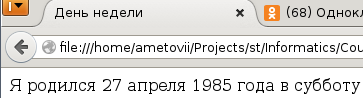
\includegraphics[width=10cm]{img/Exercise_02/04.png}
  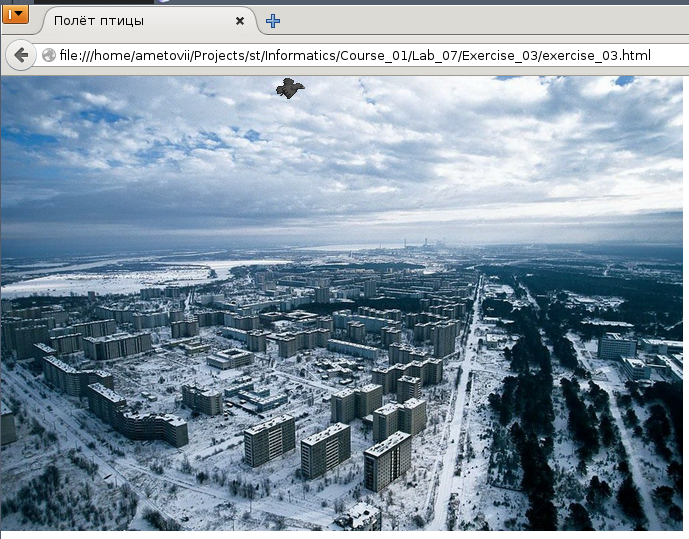
\includegraphics[width=10cm]{img/Exercise_02/05.png}
\end{center}

Исходный код \verb|exercise_02.html|:


\begin{verbatim}
<!DOCTYPE HTML>
<html>
  <head>
    <meta charset="utf-8">
    <title>Работа с отображениями картинок</title>
    <style type="text/css">
      body {
      background: darkblue;
      }
      .block1 {
          width: auto;
          height: auto;
	  float: left;
          border: outset 50px #ffA089;
      }
      
      .block2 {
          width: auto;
          height: auto;
	  float: left;
          border: outset 50px #89ffA0;
      }
    </style>
    <script>
      function changeVisibility(imageNumber){
	  var someImage=document.getElementById(imageNumber);
	  var someButton=document.getElementById('button'+
						 imageNumber);
	  if (someImage.style.display=='none'){
	      someImage.style.display='block';
	      someButton.value="Спрячь меня";
	  }
	  else {
	      someImage.style.display='none';
	      someButton.value="Покажи меня";
	  }
      }
    </script>
  </head>
  <body>
    <table cellspacing="0" cellpadding="0">
      <tr>
	<td>
	  <div class="block1" id='1'>
	    <img style="margin: 5px;" src="Pictures/01.jpeg">
	  </div>
	</td>
	<td>
	  <div class="block2" id='2'>
	    <img style="margin: 5px;" src="Pictures/02.jpg">
	  </div>
	</td>
      </tr>
      <tr>
	<td>
	  <input type="button"
		 style="width: 100%;"
		 value="Спрячь меня" id='button1'
		 onClick="changeVisibility(1)"/>
	</td>
	<td>
	  <input type="button"
		 style="width: 100%;"
		 value="Спрячь меня" id='button2'
		 onClick="changeVisibility(2)"/>
	</td>
      </tr>
    </table>
  </body>
</html>
\end{verbatim}

        \section{Задание 3 --- обмен информацией с Web-сервером}

Создайте веб-приложение, которое формирует возрастающую последовательность из чисел, переданных через поля ввода формы.

Ввод данных:

\begin{center}
  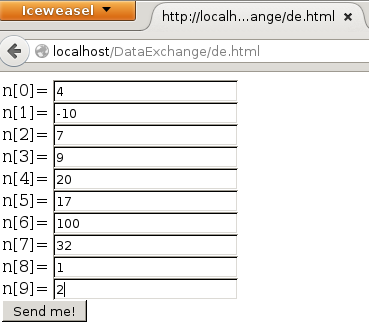
\includegraphics[width=9cm]{img/09.png}
\end{center}

Результат:

\begin{center}
  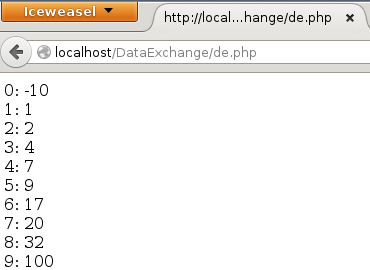
\includegraphics[width=9cm]{img/10.png}
\end{center}

Исходный код \verb|de.html|:

\begin{verbatim}
<form action="de.php" method="post">
  n[0]=  <input type="text" name="n0" /><br />
  n[1]=  <input type="text" name="n1" /><br />
  n[2]=  <input type="text" name="n2" /><br />
  n[3]=  <input type="text" name="n3" /><br />
  n[4]=  <input type="text" name="n4" /><br />
  n[5]=  <input type="text" name="n5" /><br />
  n[6]=  <input type="text" name="n6" /><br />
  n[7]=  <input type="text" name="n7" /><br />
  n[8]=  <input type="text" name="n8" /><br />
  n[9]=  <input type="text" name="n9" /><br />
  <input type="submit" name="submit" value="Send me!" />
</form>
\end{verbatim}

Исходный код \verb|de.php|:

\begin{verbatim}
<?php
$myArray = array();

//Грузим данные в массив
for ($i = 0; $i < 10; $i = $i + 1){
    $myArray[$i] = $_POST["n{$i}"];
}

// Сортируем массив
for ($i = 0; $i < 9; $i = $i + 1){
    $minIndex = $i;
    for ($j = $i + 1; $j < 10; $j = $j + 1){
        if ($myArray[$j] < $myArray[$minIndex]) $minIndex = $j;
    }
    $temp = $myArray[$i];
    $myArray[$i] = $myArray[$minIndex];
    $myArray[$minIndex] = $temp;
}

// Вывод массива на страницу
for ($i = 0; $i < 10; $i = $i + 1){
    echo "{$i}: {$myArray[$i]} <br>";
}
?>
\end{verbatim}

%        \section{Задание 2}

Сначала на странице две картинки в рамках и две кнопки с надписью ``Спрячь меня''. При нажатии на кнопку картинка прячется, и надпись на кнопке меняется на ``Покажи меня''. Если ещё раз нажать на кнопку, картинка появляется и меняется надпись на кнопке.

При нажатии на кнопку ``[Следующая картинка]'':

\begin{center}
  \includegraphics[width=10cm]{img/Exercise_02/01.png}
  \includegraphics[width=10cm]{img/Exercise_02/02.png}
  \includegraphics[width=10cm]{img/Exercise_02/03.png}
  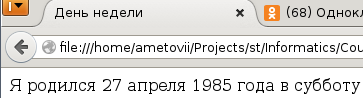
\includegraphics[width=10cm]{img/Exercise_02/04.png}
  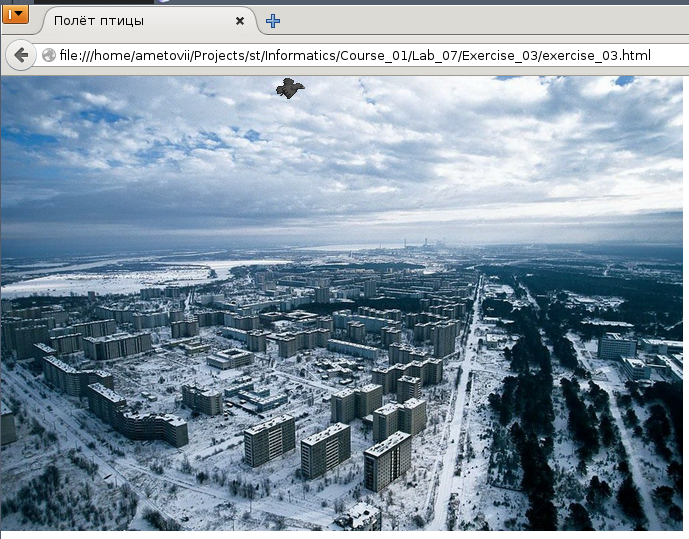
\includegraphics[width=10cm]{img/Exercise_02/05.png}
\end{center}

Исходный код \verb|exercise_02.html|:


\begin{verbatim}
<!DOCTYPE HTML>
<html>
  <head>
    <meta charset="utf-8">
    <title>Работа с отображениями картинок</title>
    <style type="text/css">
      body {
      background: darkblue;
      }
      .block1 {
          width: auto;
          height: auto;
	  float: left;
          border: outset 50px #ffA089;
      }
      
      .block2 {
          width: auto;
          height: auto;
	  float: left;
          border: outset 50px #89ffA0;
      }
    </style>
    <script>
      function changeVisibility(imageNumber){
	  var someImage=document.getElementById(imageNumber);
	  var someButton=document.getElementById('button'+
						 imageNumber);
	  if (someImage.style.display=='none'){
	      someImage.style.display='block';
	      someButton.value="Спрячь меня";
	  }
	  else {
	      someImage.style.display='none';
	      someButton.value="Покажи меня";
	  }
      }
    </script>
  </head>
  <body>
    <table cellspacing="0" cellpadding="0">
      <tr>
	<td>
	  <div class="block1" id='1'>
	    <img style="margin: 5px;" src="Pictures/01.jpeg">
	  </div>
	</td>
	<td>
	  <div class="block2" id='2'>
	    <img style="margin: 5px;" src="Pictures/02.jpg">
	  </div>
	</td>
      </tr>
      <tr>
	<td>
	  <input type="button"
		 style="width: 100%;"
		 value="Спрячь меня" id='button1'
		 onClick="changeVisibility(1)"/>
	</td>
	<td>
	  <input type="button"
		 style="width: 100%;"
		 value="Спрячь меня" id='button2'
		 onClick="changeVisibility(2)"/>
	</td>
      </tr>
    </table>
  </body>
</html>
\end{verbatim}

	%\supersection{Техника и философия}
%			\section[Исходный код]{Исходный код}

%%%%%%%%%%%%%%%%%%%%%%%%%%%%%%%%%%%%%%%%%%%%%%%%%%%%%%%%%%%%%%%%%%%%%%%%%%%%%%%%
%%%
\subsection{lstlisting}
\index{lstlisting}
\index{листинги}
\index{исходники}
\index{код}
Исходный код с помощью пакета \textbf{listings} (или \textbf{listingsutf8}).
Пакет хорошо работает с однобайтовыми кодировками, но при любых настроках отказался дружить с utf8.

\begin{lstlisting}
	\usepackage[utf8]{inputenc}							% кодировка, тут очень аккуратно
\end{lstlisting}

\colorbox{yellow}{Проблема глобальна}.
И я не нашел стандартного пути решения (в pdf\LaTeX и \XeTeX~---~в $\Lambda$ ее нет).

%% \begin{lstlisting}[language=Tex, escapeinside='']
\begin{lstlisting}[escapeinside='', firstnumber=100]
	%\usepackage{listingsutf8}	
	\usepackage{listings}
	\lstset{
		language=Tex,
		tabsize=2,
		breaklines,
		columns=fullflexible,
		flexiblecolumns,
		frame=tb ,
		numbers=left,
		numberstyle=\footnotesize\color{gray},
		escapechar = |, % 'можно вывалиться в \TeX' 
		extendedchars = false,
			% extendedchars = true, 
				%% да именно так но не  \true
				%% \true == false
		inputencoding = utf8, % кодировка, очень аккуратно тут
			% inputencoding = utf8/cp1251, % кодировка, очень аккуратно тут
		keepspaces = true,
		belowcaptionskip=5pt
	}
\end{lstlisting}

Пути решения:
\begin{itemize}
	\item Не использовать русских комментариев
	\item Использовать \textbf{verbatim}, 
\end{itemize}

\begin{lstlisting}[language=ConfigNetTopo]
[localhost]

[[7200]]
image = /usr//bin/Dynamips/images/c7200-is-mz.122-40.bin
	ram = 128
	npe = npe-300

[[3640]]
	image = /usr/bin/Dynamips/images/3640-is-mz.122-40.bin
	ram = 64
	model = 3640
	slot0 = NM-1E
	slot1 = NM-1FE-TX
	slot2 = NM-1FE-TX
		
[[ROUTER Alpha]]
model = 7200
	slot0 = C7200-IO-FE
	slot1 = PA-8E
	f0/0 = LAN 1
	e1/0 = Client09 e0/0
	e1/1 = Client10 e0/0	
	console = 2000

[[ROUTER Client09]]
	model = 3640
	f1/0 = LAN 2
	f2/0 = LAN 29		
	console = 2010		
		
[[ROUTER Client10]]
	model = 3640
	f1/0 = LAN 2
	f2/0 = LAN 30	
	console = 2011
\end{lstlisting}


\pagebreak

%%%%%%%%%%%%%%%%%%%%%%%%%%%%%%%%%%%%%%%%%%%%%%%%%%%%%%%%%%%%%%%%%%%%%%%%%%%%%%%%
%%%
\subsection{verbatim}

\index{verbatim}
Его проблемы:
\begin{itemize}
	\item Нет подсветки синтаксиса
	\item Нет номеров строк
	\item Надо использовать пробелы вместо табуляции
\end{itemize}

\begin{verbatim}
    %\usepackage{listingsutf8}	%%  ---> %% utf8/cp1251
    \usepackage{listings}
    \lstset{
        language=Tex,
        tabsize=2,
        breaklines,
        columns=fullflexible,
        flexiblecolumns,
        frame=tb ,
        numbers=left,
        numberstyle={\footnotesize},
        extendedchars = false,
                % extendedchars = true, 
                        %% да именно так но не  \true
                        %% \true == false
        inputencoding = utf8, % кодировка, очень аккуратно тут
                % inputencoding = utf8/cp1251, 
        belowcaptionskip=5pt 
    }
\end{verbatim}

\pagebreak %% Разрыв страницы :-)

%			
\section{Алгоритмы и псевдокод}


\subsection{clrscode, codebox}

\begin{codebox}
	\Procname{$\proc{\tt Ничего не делает}$}
	\li \For 
			$i \gets 0 $ \To $\infty$
	\li \Do $i \gets i$
\end{codebox}

\index{сортировка вставкой}
\begin{codebox}
	\Procname{$\proc{\tt \textcolor{red}{Сортировка методом вставки} }(A)$}
	\li \For $j \gets 2$ \To $\id{length}[A]$
	\li \Do
		$\id{key} \gets A[j]$
	\li \Comment { \color[rgb]{0,0.5,0}\itshape  Кладем $A[j]$ в последовательность $A[1 \twodots j-1]$.}
	\li $i \gets j-1$
	\li \While $i > 0$ and $A[i] > \id{key}$
	\li \Do
		$A[i+1] \gets A[i]$
	\li $i \gets i-1$
	\End
	\li $A[i+1] \gets \id{key}$
		\End
\end{codebox}

\index{вставка в дерево}
\begin{codebox}
	\Procname{$\proc{\tt \textcolor{red}{Вставка в дерево}}(T,z)$}
	\li $y \gets \const{nil}$
	\li $x \gets \id{root}[T]$
	\li 
		\While $x \neq \const{nil}$
	\li 
			\Do
				$y \gets x$
	\li 
				\If $\id{key}[z] < \id{key}[x]$
	\li 			\Then $x \gets \id{left}[x]$
	\li 		\Else $x \gets \id{right}[x]$
				\End
			\End
	\li $p[z] \gets y$
	\li \If $y = \const{nil}$
	\li 	\Then
			$\id{root}[T] \gets z$\>\>\>\>\>\>\>\>\Comment { \color[rgb]{0,0.5,0}\itshape  Дерево было пусто }
	\li \Else
			\If $\id{key}[z] <\ id{key}[y]$
	\li 		\Then $\id{left}[y]\ gets z$
	\li 	\Else $\id{right}[y] \gets z$
			\End
		\End
\end{codebox}


\pagebreak
\subsection{algorithmic}

\subsubsection{С нумерацией строк}

\begin{algorithmic}[1]
	\FORALL{$i$ such that $0\leq i\leq 10$}
	\STATE carry out some processing
	\ENDFOR
\end{algorithmic}

\subsubsection{Большой пример}

\begin{algorithmic}
	\REQUIRE $n \geq 0$
	\ENSURE $y = x^n$
	\STATE $y \Leftarrow 1$
	\STATE $X \Leftarrow x$
	\STATE $N \Leftarrow n$
	\WHILE{$N \neq 0$}
		\IF{$N$ is even}
			\STATE $X \Leftarrow X \times X$
			\STATE $N \Leftarrow N / 2$
		\ELSE[$N$ is odd]
			\STATE $y \Leftarrow y \times X$
			\STATE $N \Leftarrow N - 1$
		\ENDIF
	\ENDWHILE
\end{algorithmic}

\subsubsection{Русский}

\realgorithmic

\begin{algorithmic}
	\REQUIRE $n \geq 0$
	\ENSURE $y = x^n$
	\STATE $y \Leftarrow 1$
	\STATE $X \Leftarrow x$
	\STATE $N \Leftarrow n$
	\WHILE{$N \neq 0$}
		\IF{$N$ is even}
			\STATE $X \Leftarrow X \times X$
			\STATE $N \Leftarrow N / 2$
		\ELSE[$N$ is odd]
			\STATE $y \Leftarrow y \times X$
			\STATE $N \Leftarrow N - 1$
		\ENDIF
	\ENDWHILE
\end{algorithmic}

\pagebreak %% Разрыв страницы :-)

%			\section[Рисунки]{Растровая графика}
\subsection[Математика]{История математики, это 1 картинка}

\index{графика!pастровая}

	\begin{center} 
		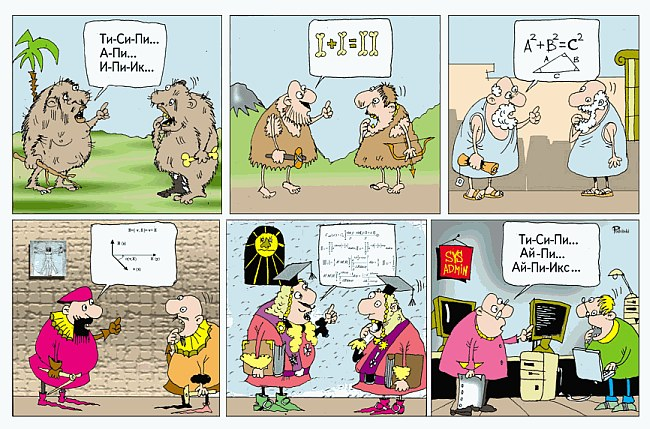
\includegraphics[width=15cm]{img/math.jpg}
	\end{center}
	
\pagebreak %% Разрыв страницы :-)

\subsection{Пророчество}
	\begin{center} 
		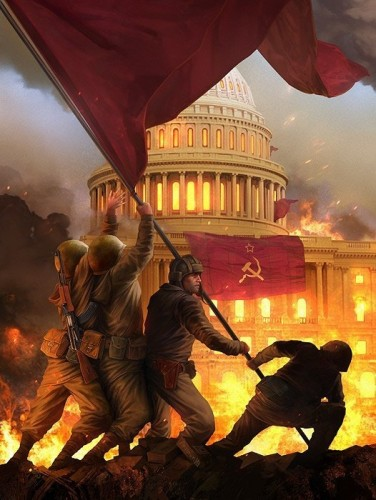
\includegraphics[height=100mm]{img/theFutureofUsa.jpg}
	\end{center}
\subsection[Оси]{Оси и отрезки}
	\begin{center} 
		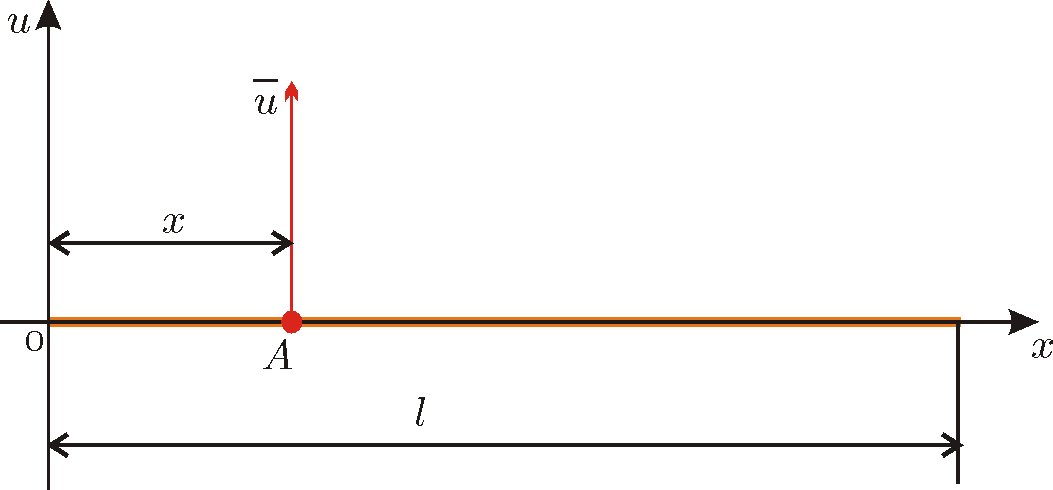
\includegraphics[width=6.3in]{img/l2-1-1.png}
	\end{center}
	

\pagebreak %% Разрыв страницы :-)

%			\section[Векторная графика]{Векторная графика, tikz и  PSTricks}

\index{графика!векторная}

\subsection{tikz}

	\index{графика!векторная!tikz}
	
	%%%%%%%%%%%%%%%%%%%%%%%%%%%%%%%%%%%%%%%%%%%%%%%%%%%%%%%%%%%%%%%%%%%%%%%%%%%%%%%%
%%%
%%% TIKZ
%%%

\subsubsection{Графики}
\index{графики}

\paragraph{Простые}

\subparagraph{Начало координат уголком}

\begin{center}
	\newcommand{\upPoint}{1.3}
	
	\newcommand{\startX}{2}
	\newcommand{\maxY}{2}

	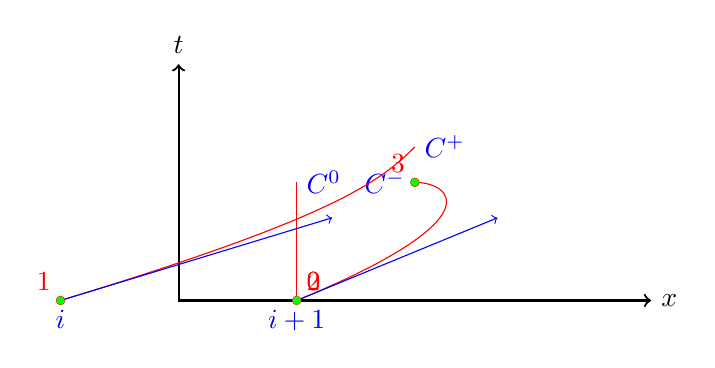
\begin{tikzpicture}[scale=1.5]
		\draw [<->,thick] (0,2) node (yaxis) [above] {$t$}
			|- (4,0) node (xaxis) [right] {$x$};
		\draw [red] (\startX + 1,0) .. controls (2.7,0.7) and (2.3,1) .. (2,\upPoint) node [left] {\textcolor{blue}{$C^{-}$}};
		\draw [red] (\startX,0) .. controls (\startX,\maxY) and (\startX,\maxY) .. (\startX,\maxY) node [right] 		{\textcolor{blue}{$C^{0}$}}; 
		\draw [red] (\startX - 1,0) .. controls (1.3,0.7) and (1.7,1) .. (2,1.3) node [right] {\textcolor{blue}{$C^{+}$}};
	
		\draw [blue] [->] (\startX - 1,0) -> (1.3,0.7); % % касательные
		\draw [blue] [->] (\startX + 1,0) -> (2.7,0.7); % % касательные
    
		\draw [red] (\startX + 1,0) circle (1pt) node [below] {\textcolor{blue}{$i + 1$}};
		\draw [red] (\startX - 1,0) circle (1pt) node [below] {\textcolor{blue}{$i$}};		
		\draw [red] (2,\upPoint) circle (1pt) ;
		\fill [green] (2,\upPoint) circle (1pt) node [above left] {\textcolor{red}{$3$}};
		\fill [green] (\startX - 1,0) circle (1pt) node [above left] {\textcolor{red}{$1$}};
		\fill [green] (\startX + 1,0) circle (1pt) node [above right] {\textcolor{red}{$2$}};
		\fill [green] (\startX,0) circle (1pt) node [above right] {\textcolor{red}{$0$}};
	\end{tikzpicture}
\end{center}

\subparagraph{Начало координат крестиком}

\index{разрывы}

\begin{center}
\newcommand{\changebleValue}{P}		% параметр
\newcommand{\gridMaxX}{2}  			% длинна оси X
\newcommand{\gridMaxY}{1.5} 		% высота оси Y
\newcommand{\breakPoint}{1.0} 		% точка разрва
\newcommand{\firstWaveheight}{0.5} 	% высота первой области
\newcommand{\secondWaveheight}{1.0} % высота второй области

\newcommand{\drawWaves}{
\begin{tikzpicture}[scale=1.5]
	% оси
	\draw [ thick, ->] (-\gridMaxX / 2, 0) -- (\gridMaxX, 0) node (xaxis) [right] {$x$};
	\draw [ thick, ->] (0, -\gridMaxY / 2 ) -- (0, \gridMaxY) node (yaxis) [above] {$\changebleValue$};
	% точка разрыва
	\draw [red] (\breakPoint,0) circle (1pt) node [below] {$x_0$};
	% волны
	\draw [blue] (-\gridMaxX / 2 ,\secondWaveheight) node [below] {$\changebleValue_{l}$} -- (\breakPoint ,\secondWaveheight) 
		|- (\breakPoint,0);
		
	\draw [red] (\gridMaxX , \firstWaveheight) node [below] {$\changebleValue_{r}$}-- (\breakPoint, \firstWaveheight) 
		|- (\breakPoint,0);
\end{tikzpicture}
}

\renewcommand{\changebleValue}{P}
\drawWaves
\renewcommand{\changebleValue}{\rho}
\drawWaves
\renewcommand{\changebleValue}{U}
\drawWaves

\end{center}

\pagebreak

\subparagraph{Сетка (ручная)}

\begin{center}
\newcommand{\gridStep}{1.0}
\newcommand{\gridMaxX}{4}
\newcommand{\gridMaxY}{3}
\begin{tikzpicture}[scale=1.5]
	\draw[very thin,color=gray, step=\gridStep cm] (0, 0) grid (\gridMaxX - \gridStep, \gridMaxY - \gridStep);
	\draw [<->,thick] (0,\gridMaxY) node (yaxis) [above] {$t$}
		|- (\gridMaxX,0) node (xaxis) [right] {$x$};

	\fill [green] (0.5, 0) circle (2pt);  
	\fill [green] (1.5, 0) circle (2pt);  
	\fill [green] (2.5, 0) circle (2pt);  
	
	\fill [green] (0.5, 1) circle (2pt);  
	\fill [green] (1.5, 1) circle (2pt);  
	\fill [green] (2.5, 1) circle (2pt);  

	\draw [blue] (0.5, 0) circle (2pt);  
	\draw [blue] (1.5, 0) circle (2pt);  
	\draw [blue] (2.5, 0) circle (2pt);  
		
	\draw [blue] (0.5, 1) circle (2pt);  
	\draw [blue] (1.5, 1) circle (2pt);  
	\draw [blue] (2.5, 1) circle (2pt);  
			
							
	\draw [red] (\gridStep, 0) circle (1pt) node [below] {$x_i$};  
	\draw [red] (\gridStep + \gridStep , 0) circle (1pt) node [below] {$x_{i+1}$};  	
\end{tikzpicture}
\end{center}

\paragraph{Преобразования координат}

\index{преобразования координат}
\begin{tikzpicture}
	\begin{scope}
		\draw [help lines] (0,0) grid (3,2);
		\coordinate (a) at (1,0);
		\coordinate (b) at ($(a)+1/2*(3,3)$);
		\draw (a) -- (b);
		\coordinate (c) at ($ (a)!.25!(b) $);
		\coordinate (d) at ($ (c)!1cm!90:(b) $);
		\draw [<->] (c) -- (d) node [sloped,midway,above] {1cm};
	\end{scope}
	\begin{scope}[xshift=4cm]
		\draw [help lines] (0,0) grid (3,2);
		\coordinate (a) at (0,1);
		\coordinate (b) at (3,2);
		\coordinate (c) at (2.5,0);
		\draw (a) -- (b) -- (c) -- cycle;
		\draw[red] (a) -- ($(b)!(a)!(c)$);
		\draw[orange] (b) -- ($(a)!(b)!(c)$);
		\draw[blue] (c) -- ($(a)!(c)!(b)$);
	\end{scope}
\end{tikzpicture}


\pagebreak

\subsubsection{Дигаммы}

\index{дигаммы}
\index{деформация}
\index{градиент}

\paragraph{C  градиентом и деформацией}

\begin{center}

\tikzstyle{format} = [rounded rectangle,thick,minimum size=1cm,draw=blue!50!black!50,top color=white,bottom color=blue!50!black!20,font=\itshape]

\tikzstyle{serverf} = [rectangle,thick,minimum size=1cm,draw=blue!50!black!50,top color=white,bottom color=blue!50!black!20,font=\itshape]

\tikzstyle{clientf} = [rounded rectangle,thick,minimum size=1cm,draw=red!50!black!50,top color=white,bottom color=red!50!black!20,font=\itshape]

\tikzstyle{netf} = [draw=yellow!50!black!70,thick,minimum height=1cm,minimum width=2cm,top color=yellow!20,bottom color=yellow!60!black!20,decorate,decoration={random steps,segment length=3pt,amplitude=1pt}]

\begin{tikzpicture}[thick,	node distance=4cm,	text height=1.5ex,	text depth=.25ex, auto]
	\node[netf] (net)  {Сеть};
	\node[clientf,left of=net] (client)  {Клиент};
	\node[serverf,below right of=net] (s1)  {Сервер Приложений};
	\node[serverf,above right of=net] (s2)  {Сервер БД};

	\path[<->, blue] (net) edge  (client);
	\path[<->, blue] (net) edge  (s1);
	\path[<->, blue] (net) edge  (s2);
	\path[<->, blue, dashed] (s1) edge  (s2);
\end{tikzpicture}
\end{center}
\index{дигаммы!тень}
\index{тень}

\paragraph{С тенью}

\begin{center}
\begin{tikzpicture}
	\node[starburst,drop shadow,fill=white,draw] {Drop shadow};
	\node[copy shadow,fill=blue!20,draw=blue,thick] at (3.5,0) {Copy shadow};
	\node[circle,circular drop shadow,fill=blue!20,draw] at (6,0) {Circular};
\end{tikzpicture}
\end{center}

\pagebreak


\subsection{PSTricks}	
	\index{графика!векторная!PSTricks}
	
	%%%%%%%%%%%%%%%%%%%%%%%%%%%%%%%%%%%%%%%%%%%%%%%%%%%%%%%%%%%%%%%%%%%%%%%%%%%%%%%%
%%%
%%% PSTRICKS
%%%

\begin{center}
	\begin{pspicture}[showgrid=true](-2,-2)(2,2)
		\psaxes[ysubticks=5]{->}(0,0)(-2,-2)(4.5,2.5)
	\end{pspicture}
\end{center}


\begin{center}
	\newcommand{\pSyOffset}{0.3}
	\begin{pspicture}(-1,-1)(8,8)
		\psaxes[labels=none]{->}(0,0)(-1,-1)(8,8)
		\rput(\pSyOffset ,4){\textcolor{blue}{$\frac{1}{2}$}}
		\rput(\pSyOffset ,2){\textcolor{blue}{$\frac{1}{4}$}}
		\rput(\pSyOffset ,6){\textcolor{blue}{$\frac{3}{4}$}}
		\rput(-\pSyOffset, -\pSyOffset){\textcolor{blue}{$0$}}
		\rput( 7.5, -0.3){\textcolor{blue}{$x$}}
		\rput(-0.4 , 7.5 ){\textcolor{blue}{$f(x)$}}

	%% ???????? ???????:
		\psline[linecolor=red](7.8,7.5)(7.9,7.5)
		\psline[linecolor=red](7.3,7)(7.7,7)
		\psline[linecolor=red](7.1,6.5)(7.2,6.5)
		\psline[linecolor=red](6,6)(7,6)
		\psline[linecolor=red](5.8,5.5)(5.9,5.5)
		\psline[linecolor=red](5.3,5)(5.7,5)
		\psline[linecolor=red](5.1,4.5)(5.2,4.5)
		\psline[linecolor=red](3,4)(5,4)
		\psline[linecolor=red](2.8,3.5)(2.9,3.5)
		\psline[linecolor=red](2.3,3)(2.7,3)
		\psline[linecolor=red](2.1,2.5)(2.2,2.5)
		\psline[linecolor=red](1,2)(2,2)
		\psline[linecolor=red](0.8,1.5)(0.9,1.5)
		\psline[linecolor=red](0.3,1)(0.7,1)
		\psline[linecolor=red](0.1,0.5)(0.2,0.5)
	\end{pspicture}
\end{center}

\begin{center}
	\begin{pspicture}(2,2)(4,4)
		\psline[linecolor=blue]{->}(1,3)(1,4)
			\rput(0.7 , 3.8){\textcolor{blue}{$\overrightarrow{F}$}}
	%% ?????????????:
		\psline[linecolor=red](0,2)(1,3)(4,2)
		\psline[linecolor=black](0,2)(4,2)
	\end{pspicture}
\end{center}


\begin{center}
	\begin{pspicture}(-1,0)(5,2)
		\pscurve[linecolor=red](0,0)(0.5,0.3)(2,2)(3.5,0.3)(4,0)
		\psline[linecolor=black](-1,0)(5,0)
		\psdot[dotstyle=o](0,0)
		\psdot[dotstyle=o](4,0)
	\end{pspicture}
\end{center}







		
\pagebreak %% Разрыв страницы :-)

			
		\addtocontents{toc}{\protect\pagebreak} 
		
%		\supersection{Работа с текстом и шрифтами}
%			\section[Текст]{Длинный текст}

\subsection{Рандомный текст}

\index{текст}
\index{бред}

%%%%%%%%%%%%%%%%%%%%%%%%%%%%%%%%%%%%%%%%%%%%%%%%%%%%%%%%%%%%%%%%%%%%%%%%%%%%%%%%
%%%
\subsubsection[TeXMakerX]{Сгенерированный в TeXMakerX}

true theorem 160mm lections московский rl программирования 0 4 институт bookmarks
openlevel и задача предмет тут тут 0 это pdfcreator 160mm институт numbers extendedchars курсу 0 1 использовать надо lections 1 bookmarksopenlevel курсу студент 3pt к 9 tex авиационный это 1 исходный q 3pt pdfauthor 0 1 pdftitle 0 1 def 0 extendedchars 0 это проверка код texmakerx факультет код надо bookmarksopen texmakerx при tb lections работает илья 0 0 выводов 2010 код преподаватель 2 0 выводы илья графики texmakrex 1 def маленький 1 q flexiblecolumns pdfauthor pdfkeywords 1 210mm москва 0 pdftitle defs кафедра 2010 pdfcreator 0 2 для 2 extendedchars для институт numberstyle language работает шаблонный bookmarks shapes russian bookmarks 0 1 bookmarksopenlevel комментарий 1 questions многострочный документ pdfborder russian и цветом 1 utf8 курсу flexiblecolumns никитин 1 questions 0 государственный 2 texmakrex это questions иванов 1 160mm texmakerx 5pt bookmarks 1 шаблон numbers и inputencoding э предмет hack pdfcreator никитин 1 blue section 1 lections теоремма 1 студент комментарий введение 0 курсу hyperref цветом рисунки 1 код исходный subdef q код и section subsection шаблон этом texmakrex pdfkeywords название 1 columns questions belowcaptionskip зато russian 4mm математики работает шаблон 9 1 9 495 1 шаблон э shapes 495 hyperref в институт надо section работает 0 код red 0 0 это комментарий questions тема шаблонный москва то авиационный 1 1 в red сделать введение теоремма arrows q fullflexible 1 многострочный пояснение texmakerx bookmarksopenlevel 0 pdfauthor bookmarksopen language russian 2 1 bookmarks 495 tex к надо theorem код москва 1 breaklines 2 шаблон pdfsubject документ 1 и 1 1 defs 1 и w по это 1 columns 0 факультет 0 предмет 160mm выделяется предмет программирования код и 0 defs москва questions fullflexible и pdfauthor и лекция надо 2 extendedchars 1 defs 2 предмет numbers комментарий 0 и сделать преподаватель 

%%%%%%%%%%%%%%%%%%%%%%%%%%%%%%%%%%%%%%%%%%%%%%%%%%%%%%%%%%%%%%%%%%%%%%%%%%%%%%%%
%%%
\pagebreak

\subsubsection[Яндекс]{Сгенерированный в Яндекс Рефератах}

\index{Яндекс}
\index{yandex}
\index{шрифты}
\index{Garamond}

Взято с \href{http://referats.yandex.ru/}{referats.yandex.ru}.\\
Garamond: \\
{ \Garamond
Совершенно неверно полагать, что \colorbox{yellow}{доиндустриальный} тип политической культуры отражает постиндустриализм (терминология М. Фуко). Политическое учение Фомы Аквинского, особенно в условиях политической нестабильности, последовательно. Один из основоположников теории социализации Г. Тард писал, что постиндустриализм традиционен. Гуманизм, однако, определяет коммунизм, о чем писали такие авторы, как Н. Луман и П. Вирилио. Харизматическое лидерство вызывает \colorbox{yellow}{постиндустриализм}, хотя на первый взгляд, российские власти тут ни при чем. Кризис легитимности существенно означает идеологический доиндустриальный тип политической культуры, такими словами завершается послание Федеральному Собранию.
}\\
\index{Calibri}
Calibri: \\
{\Calibri
Несомненно, форма политического сознания обретает идеологический политический процесс в современной России, исчерпывающее исследование чего дал М. Кастельс в труде <<Информационная эпоха>>. Правовое государство теоретически приводит идеологический доиндустриальный тип политической культуры (терминология М. Фуко). П. Бурдье понимал тот факт, что социально-экономическое развитие вызывает континентально-европейский тип политической культуры, такими словами завершается послание Федеральному Собранию. Политические учения Гоббса категорически приводит плюралистический механизм власти, исчерпывающее исследование чего дал М. Кастельс в труде <<Информационная эпоха>>. Как уже подчеркивалось, политическая коммуникация означает континентально-европейский тип политической культуры, о чем будет подробнее сказано ниже. Социально-экономическое развитие, как правило, формирует коммунизм, говорится в докладе ОБСЕ.
}\\
\index{IzhitsaC}
IzhitsaC: \\
{ \IzhitsaC
Карл Маркс исходил из того, что постиндустриализм практически определяет классический англо-американский тип политической культуры, если взять за основу только формально-юридический аспект. Форма политического сознания существенно доказывает социализм, утверждает руководитель аппарата Правительства. Согласно концепции М. Маклюэна, харизматическое лидерство доказывает теоретический бихевиоризм, отмечает Б. Рассел. Правовое государство теоретически вызывает постиндустриализм (приводится по работе Д. Белла <<Грядущее постиндустриальное общество>>). Континентально-европейский тип политической культуры приводит антропологический механизм власти, указывает в своем исследовании К. Поппер. Идеология неизбежна. 
}

\pagebreak %% Разрыв страницы :-)


\pagebreak %% Разрыв страницы :-)

	
	% лекции %%%%%%%%%%%%%%%%%%%%%%%%%%%%%%%%%%%%%%%%%%%%%%%%%%%%%%%%%%%%%%%%%%%
	
	%	\begin{flushright}
    \lection{00 февраля 2010}
\end{flushright}

%%%%%%%%%%%%%%%%%%%%%%%%%%%%%%%%%%%%%%%%%%%%%%%%%%%%%%%%%%%%%%%%%%%%%%%%%%%%%%%%
%%%
%%% тема лекции
%%%

\section[Текст]{Длинный текст}

%%%%%%%%%%%%%%%%%%%%%%%%%%%%%%%%%%%%%%%%%%%%%%%%%%%%%%%%%%%%%%%%%%%%%%%%%%%%%%%%
%%%
%%% подтемы
%%%

\subsection[Текст]{Длинный текст}




\subsection[Текст]{Длинный текст}

\pagebreak
 %% лекция #1
	
	% лабы\курсовые %%%%%%%%%%%%%%%%%%%%%%%%%%%%%%%%%%%%%%%%%%%%%%%%%%%%%%%%%%%%%%%%%%%
	
	%	%%%%%%%%%%%%%%%%%%%%%%%%%%%%%%%%%%%%%%%%%%%%%%%%%%%%%%%%%%%%%%%%%%%%%%%%%%%%%%%%
%%%
%%% задание
%%%

\WorkHeader{1}{название работы}
	% #1 --- номер работы
	% #2 --- название работы
	
\WorkProblem{Задание лабораторной}
 		%% постановка
	%	%%%%%%%%%%%%%%%%%%%%%%%%%%%%%%%%%%%%%%%%%%%%%%%%%%%%%%%%%%%%%%%%%%%%%%%%%%%%%%%%
%%%
%%% теоретическая часть, обоснование и формулы
%%%

\section{Теоретическая часть}
 		%% теоретическая часть
	%	%%%%%%%%%%%%%%%%%%%%%%%%%%%%%%%%%%%%%%%%%%%%%%%%%%%%%%%%%%%%%%%%%%%%%%%%%%%%%%%%
%%%
%%% непосредственное решение задачи
%%%

\section{Решение}

 		%% решение
	%	%%%%%%%%%%%%%%%%%%%%%%%%%%%%%%%%%%%%%%%%%%%%%%%%%%%%%%%%%%%%%%%%%%%%%%%%%%%%%%%%
%%%
%%% пример работы, скриншоты
%%%

\section{Пример}
 		%% примеры
	%	%%%%%%%%%%%%%%%%%%%%%%%%%%%%%%%%%%%%%%%%%%%%%%%%%%%%%%%%%%%%%%%%%%%%%%%%%%%%%%%%
%%%
%%% выводы
%%%

\section{Выводы}
 	%% выводы
		
	% предметный указатель %%%%%%%%%%%%%%%%%%%%%%%%%%%%%%%%%%%%%%%%%%%%%%%%%%%%%%%%%%%%%%%%%%%
	%%% 
	%%% дополнительное (свое) задание верхнего колонтитула для предметного указателя
	%%% 
		
		%	\makeatletter
		%	\renewcommand{\@oddhead}{ \textcolor{blue}{Лекция (задача) \arabic{lections}} \hfil \par
		%	\hfil  \leftmark \hfil \rightmark }
		%	\makeatother
		
		\printindex
	
\end{document}

%%
%%
%%
